\section{研发概述}
\subsection{团队组建}
团队组建:
\begin{table}[H]
  \centering
  \caption{开发团队组建人员}
    \begin{tabular}{|c|ccccc|}
    \hline
    \textcolor[rgb]{ .298,  .282,  .239}{技术团队成员} & \multicolumn{1}{p{6.78em}|}{\textcolor[rgb]{ .298,  .282,  .239}{数据库后端工程师}} & \multicolumn{1}{p{5.61em}|}{\textcolor[rgb]{ .298,  .282,  .239}{ web前端工程师}} & \multicolumn{1}{p{6.11em}|}{\textcolor[rgb]{ .298,  .282,  .239}{移动前端工程师}} & \multicolumn{1}{p{5.72em}|}{\textcolor[rgb]{ .298,  .282,  .239}{视频底层工程师}} & \multicolumn{1}{p{4.165em}|}{\textcolor[rgb]{ .298,  .282,  .239}{界面设计师}} \\
    \hline
    \textcolor[rgb]{ .298,  .282,  .239}{人数} & \multicolumn{1}{c|}{\textcolor[rgb]{ .298,  .282,  .239}{1}} & \multicolumn{1}{c|}{\textcolor[rgb]{ .298,  .282,  .239}{1}} & \multicolumn{1}{c|}{\textcolor[rgb]{ .298,  .282,  .239}{2}} & \multicolumn{1}{c|}{\textcolor[rgb]{ .298,  .282,  .239}{1}} & \textcolor[rgb]{ .298,  .282,  .239}{1} \\
    \hline
    \textcolor[rgb]{ .298,  .282,  .239}{总人数} & \multicolumn{5}{c|}{\textcolor[rgb]{ .298,  .282,  .239}{6}} \\
    \hline
    \end{tabular}%
  \label{tab:kaifarenyuan}%
\end{table}%


\begin{table}[H]
  \centering
  \caption{开发团队成员基本需求}
    \begin{tabular}{|c|p{28.61em}|}
    \hline
    \textcolor[rgb]{ .298,  .282,  .239}{流程} & \textcolor[rgb]{ .298,  .282,  .239}{熟悉PSP开发流程} \\
    \hline
    \textcolor[rgb]{ .298,  .282,  .239}{交流} & \textcolor[rgb]{ .298,  .282,  .239}{能有效地和其他队员交流,从大的技术方向,到看似微小的问题} \\
    \hline
    \textcolor[rgb]{ .298,  .282,  .239}{准备} & \textcolor[rgb]{ .298,  .282,  .239}{在开会讨论之前,开始一个新功能之前、一个新项目之前,都要做好准备工作} \\
    \hline
    \textcolor[rgb]{ .298,  .282,  .239}{按时交付} & \textcolor[rgb]{ .298,  .282,  .239}{能够按照工期预算按时交付} \\
    \hline
    \textcolor[rgb]{ .298,  .282,  .239}{全力投入团队} & \textcolor[rgb]{ .298,  .282,  .239}{一些评审会议,代码复审,都要全力以赴地参加,而不是游离于团队之外} \\
    \hline
    \end{tabular}%
  \label{tab:kaifarenyuanyaoqiu}%
\end{table}%



\subsection{需求分析}
\subsubsection{运行需求}\

网课系统从网页端、手机移动端两个端口开发前端应用。

\paragraph{网页端}\

在互联网上具有独立网站,网站能够兼容现在主流类型的浏览器和其主流版本。

\paragraph{手机移动端}\

具有独立的APP软件,能够支持目前主流的Android系统和主流的iOS系统。APP能够实现和网页端同步数据,也要具有网页端相同的功能。

\subsubsection{功能需求}\

\paragraph{课程视频展示}\

在系统主界面,展示当前的精品课程和针对用户的推荐课程,并且在对应课程上展示对此课程的简单介绍。后期课程达到一定数量时,在系统主界面,展示当前所有的课程分类目录。

\paragraph{用户注册和登陆}\

系统能够提供用户的注册界面,用户提供其信息(包括用户名,密码,手机号,兴趣等)就能够在系统上注册一个能够使用的学生端账户。系统能够提供用户的登陆界面,用户提供用户名和密码就可以登陆到对应的账户并享受系统的后续服务。

\paragraph{课程视频播放}\

系统能够提供课程视频播放服务,免费课程用户可以直接播放,提供视频播放界面、课程信息界面、课程资源界面、课程目录界面,视频能够流畅播放,除网络问题外没有卡顿和失真等影响视频观看的问题。付费课程则提供前1-2分钟的试观看,试观看结束之后则要求用户进行付费,若付费成功则视频继续播放,若未完成付费则无法继续观看后段视频。视频播放界面需要有播放进度条、画质清晰度调整、播放速度调整、界面大小调整等功能。移动端还需要支持音频的独立播放。

\paragraph{课程查找}\

当用户在搜索框中输入关键字时,系统能根据用户的关键字进行搜索,找到匹配的课程视频后,将符合条件的课程视频展示给用户,包含其对应的课程信息和免费\\付费金额等信息。

\paragraph{课程购买}\

用户能够对需要付费的视频进行付费购买操作,当用户付费完成之后,该账户就享有当前课程视频的一定时间的观看权,在该时间内,用户在网页端和移动端都能够观看该视频,在移动端还支持离线下载,下载的视频仅可供移动端离线播放。用户能够查看历史购买的订单信息,包括购买时间,购买金额,所购买的课程信息和课程可使用期限等。

\paragraph{课程管理}\

系统管理员可以在后台管理课程,可以上传新的课程视频,也可删除服务器中存储的课程视频,还可以对服务器中的课程视频信息(如名称、介绍、价格等)进行更改。系统管理员能够查看系统运营业绩,即每个视频的点击量和销售量,并进行数据统计和分析。

\paragraph{用户管理}\

系统管理员可以在后台进行用户账户的增加和删除操作,还可以对用户的信息进行更改。系统管理员查看用户的流量信息,即某段时间内注册的用户量、用户的兴趣分类统计、用户的购买量等信息。

\subsubsection{非功能性需求}\

\paragraph{性能}\

该系统在一般环境(主流的电脑浏览器和手机,合适的网络环境)下,能够流畅的启动和显示,能够流畅的进行各项操作,视频播放应该流畅、不卡顿、不失真、不掉帧。系统初期需要能够承载至少1000用户量和1000G视频量。

\paragraph{可用性}\

系统的外观、界面美观简洁,操作便利简单,符合现在主流的网络用户的操作习惯,在关键操作部分给出清晰简明的提示信息,体现良好的用户友好性。

\paragraph{安全性}\

只有开发人员和维护人员才有权限查看和修改该系统的源代码,以防止程序和数据受到意外的或蓄意的存取、使用、修改、毁坏或泄密。系统进行数据传输时需要加密,防止视频等重要数据资源泄露,用户移动端的离线下载后的视频文件需要进行编码加密,防止视频非法传播和盗用。

\paragraph{可维护性}\

代码有足够的注释,清晰的结构,变量、函数等的命名具有较高的易理解性,以便修改潜伏的错误,改进性能和其他属性,增减功能等,使得后期系统能够在此系统的基础上再次进行开发。

\subsection{开发流程}
开发流程如下:
\begin{figure}[H]
	\centering
	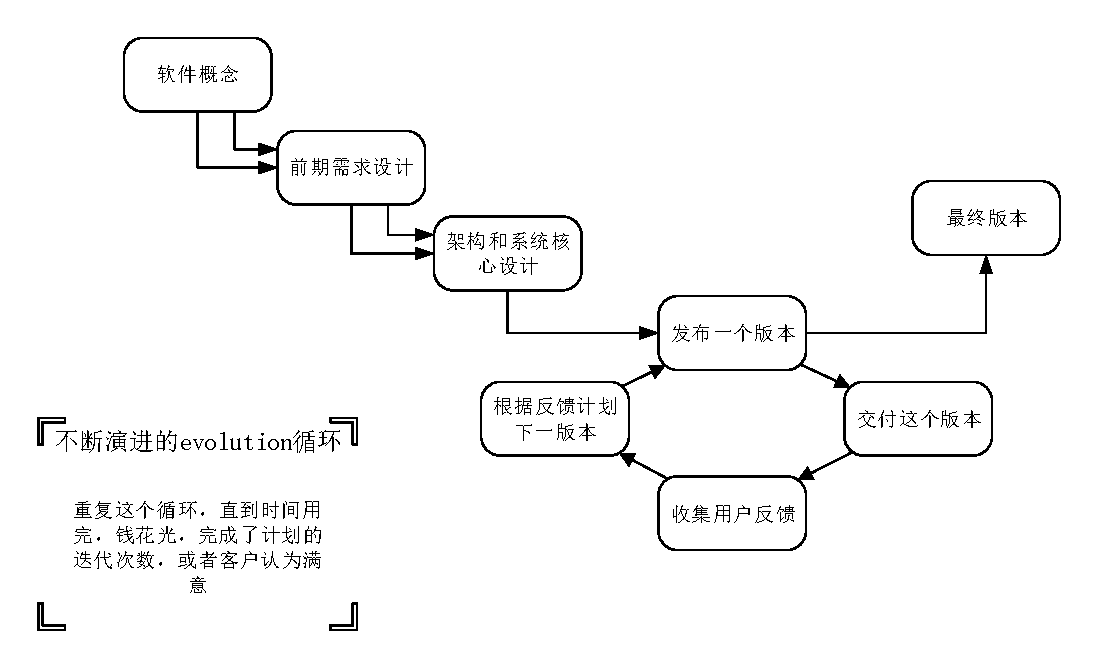
\includegraphics[width=0.9\columnwidth]{figures/system_development_process}
	%  \setlength{\abovecaptionskip}{0pt}
	%  \setlength{\belowcaptionskip}{-20pt}
	\caption{系统开发流程图}
	\label{fg:system_development_process}
\end{figure}

\subsection{用户体验}
用户体验评价标准:
\begin{table}[H]
  \centering
  \caption{用户体验评价标准}
    \begin{tabular}{|p{8.335em}|p{17.665em}|}
    \hline
    \textcolor[rgb]{ .298,  .282,  .239}{评价标准} & \textcolor[rgb]{ .298,  .282,  .239}{评价要求} \\
    \hline
    \textcolor[rgb]{ .298,  .282,  .239}{尽快提供可感触的反馈} & \textcolor[rgb]{ .298,  .282,  .239}{系统状态要有反馈,等待时间要合适} \\
    \hline
    \textcolor[rgb]{ .298,  .282,  .239}{系统界面符合用户的现实惯例} & \textcolor[rgb]{ .298,  .282,  .239}{与用户沟通使用用户语言而不是开发者语言,给用户提供必要的信息提示,减少用户的记忆负担,从而减少认知阻力} \\
    \hline
    \textcolor[rgb]{ .298,  .282,  .239}{用户有控制权} & \textcolor[rgb]{ .298,  .282,  .239}{操作失误可以回退,要让用户可以退出软件,用户可以定制显示信息的多少,还可以定制常用设置} \\
    \hline
    \textcolor[rgb]{ .298,  .282,  .239}{一致性和标准化} & \textcolor[rgb]{ .298,  .282,  .239}{对同一事物和同类操作的表示用语,各处要保持一致} \\
    \hline
    \textcolor[rgb]{ .298,  .282,  .239}{适合各种类型的用户} & \textcolor[rgb]{ .298,  .282,  .239}{要为新手和专家提供可定制化的设计,对于长期使用软件的用户,应该能够适应用户的使用习惯,让用户越用越顺手,最后产生感情上的好感和忠诚度} \\
    \hline
    \multirow{2}[2]{*}{\textcolor[rgb]{ .298,  .282,  .239}{帮助用户识别、诊断并修复错误}} & \textcolor[rgb]{ .298,  .282,  .239}{软件的关键操作要有确认提示,以便帮助用户及早消除误操作。要注意使用朴素的语言描述错误信息,错误信息要给出下一步操作提示。} \\
    \multicolumn{1}{|c|}{} & \textcolor[rgb]{ .298,  .282,  .239}{让所有的用户都可以通过电子邮件或者表单来提交反馈意见} \\
    \hline
    \textcolor[rgb]{ .298,  .282,  .239}{有必要的提示和帮助文档} & \textcolor[rgb]{ .298,  .282,  .239}{必要时提供在线帮助和帮助文档} \\
    \hline
    \end{tabular}%
  \label{tab:yhty}%
\end{table}%


\subsection{软件测试和质量保障}
\subsubsection{软件测试}\

在软件开发过程中的每一个小阶段都要进行当前已经完成的软件的测试,测试需要测试文档,包括测试设计说明书,测试用例,程序错误报告和测试报告。其中测试报告中需要按照如下要求报告bug:

\paragraph{症状:}\

即从用户的角度看,软件出了什么问题。

\paragraph{程序错误:}\

即从代码的角度看,软件的什么错误导致了软件的问题。

\paragraph{根本原因:}\

错误根源,即导致代码错误的根本原因。

\begin{figure}[H]
	\centering
	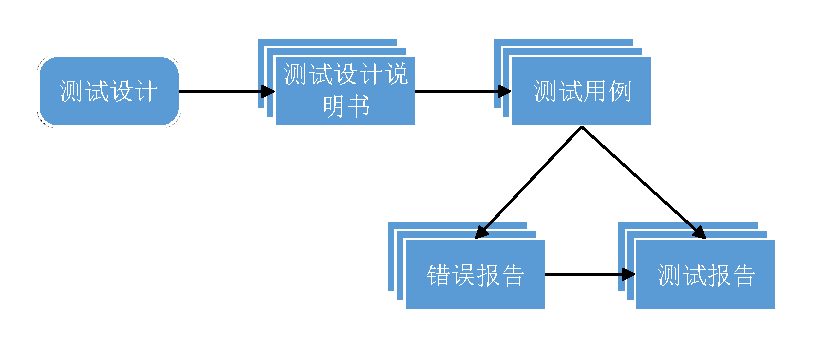
\includegraphics[width=0.9\columnwidth]{figures/test_document}
	%  \setlength{\abovecaptionskip}{0pt}
	%  \setlength{\belowcaptionskip}{-20pt}
	\caption{测试工作中的文档}
	\label{fg:test_document}
\end{figure}

\subsubsection{质量保障}\

成立软件质量保证(SQA)小组,确保开发者确实进行高质量的工作,每个开发者和维护者应对检查自己工作正确负责,每一个阶段性的工作完成之后由SQA小组审查工作的正确性和完整性,每一个阶段性的工作完成之后由SQA小组审查对应文档的完整性。

\begin{figure}[H]
	\centering
	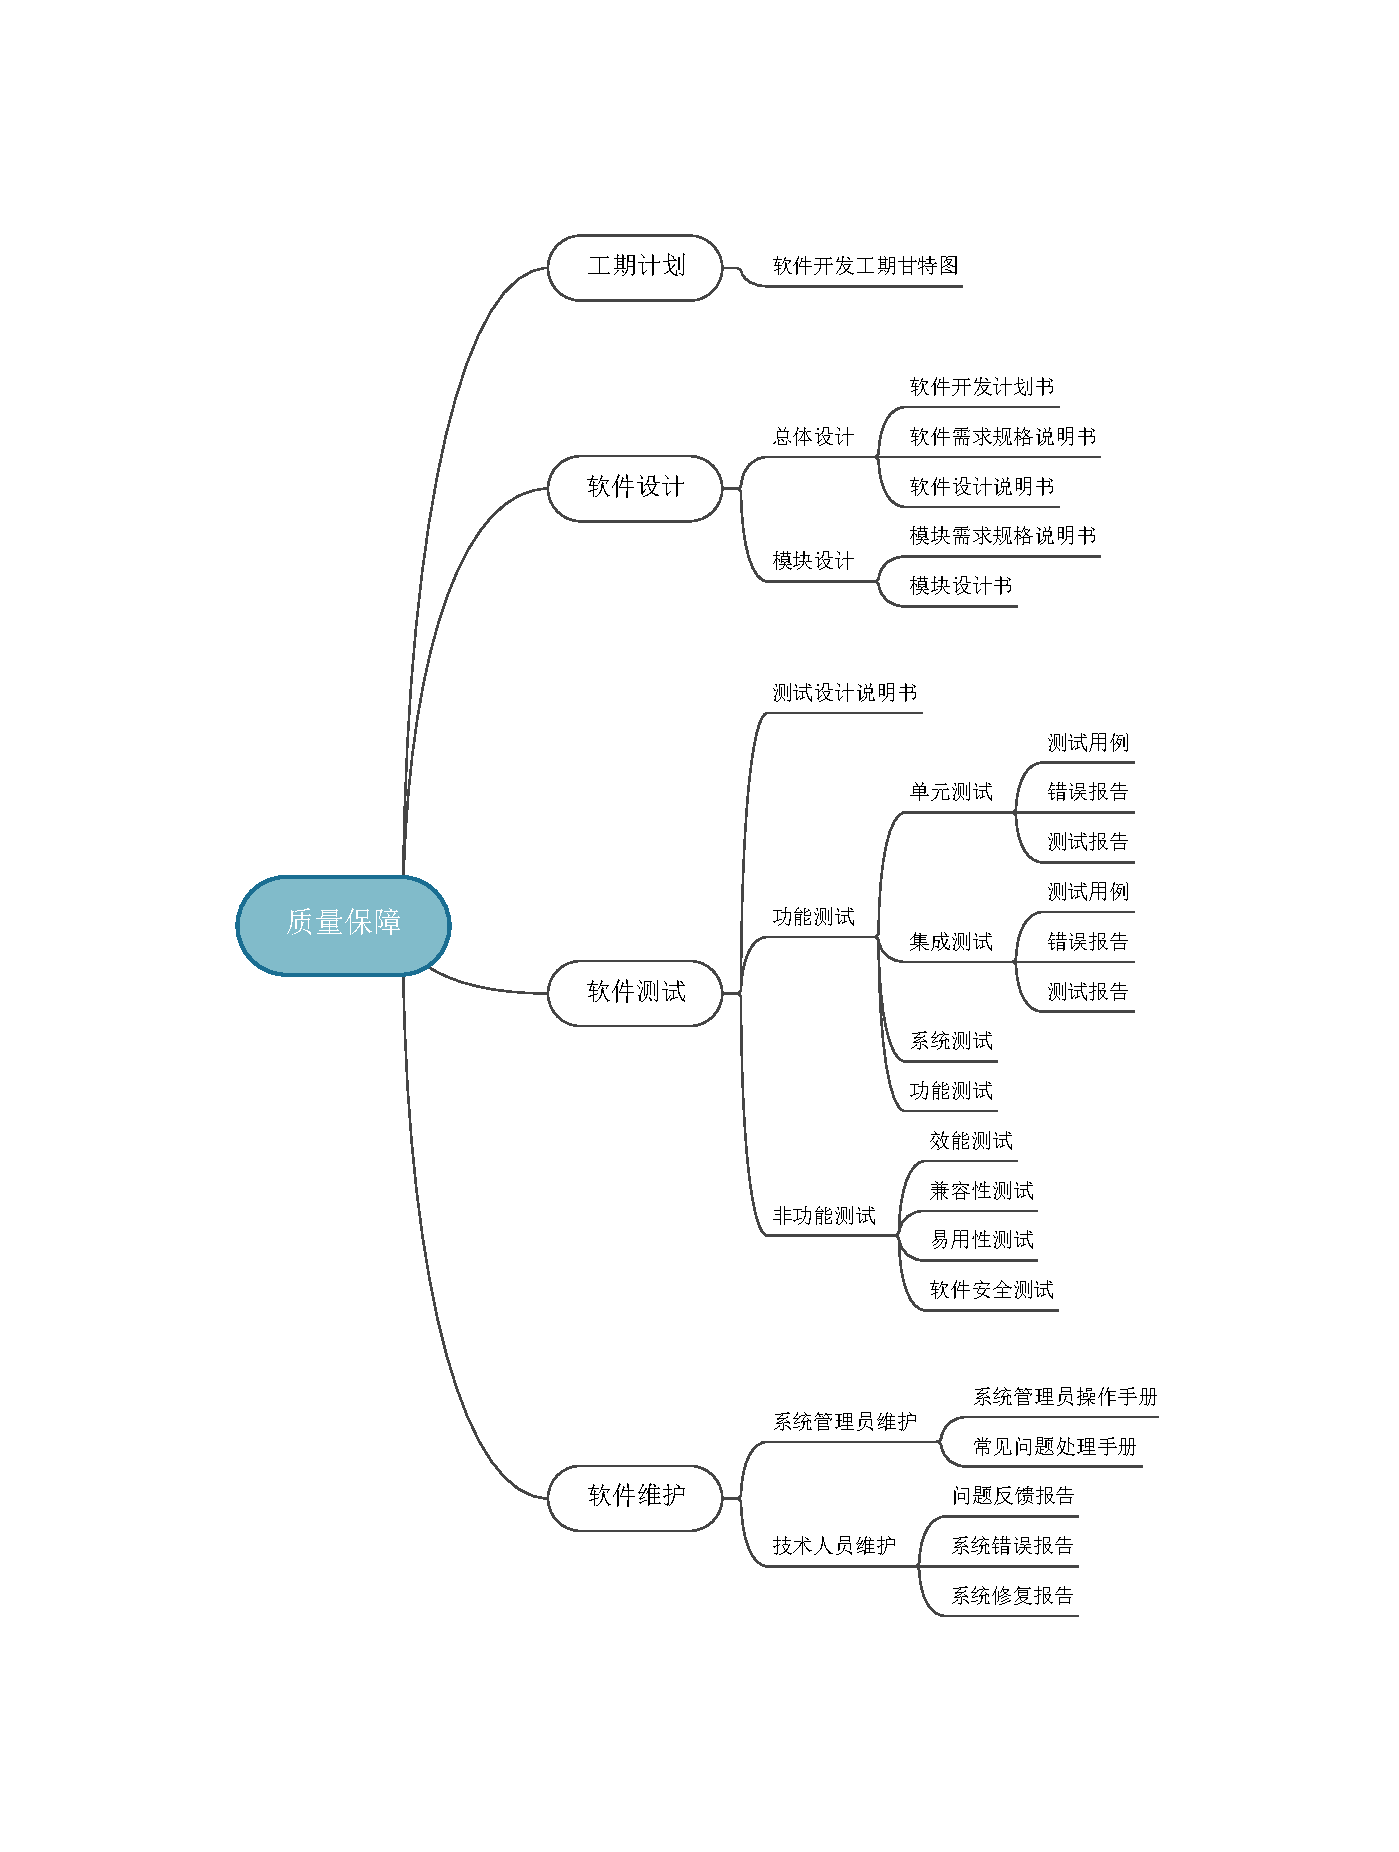
\includegraphics[width=0.9\columnwidth]{figures/software_quality_assurance}
	%  \setlength{\abovecaptionskip}{0pt}
	%  \setlength{\belowcaptionskip}{-20pt}
	\caption{软件质量保障文档审核总览}
	\label{fg:software_quality_assurance}
\end{figure}

\subsection{成本估算}
\subsubsection{硬件成本}\

以华为云在2018年6月30号的价格报表为参考标准,最终租赁版本未确定。

% Table generated by Excel2LaTeX from sheet 'Sheet1'
\begin{table}[H]
  \centering
  \caption{硬件成本估计}
    \begin{tabular}{|p{4.055em}|p{5.555em}cc|}
    \hline
    \textcolor[rgb]{ .298,  .282,  .239}{租赁项目} & \multicolumn{1}{p{5.555em}|}{\textcolor[rgb]{ .298,  .282,  .239}{服务器}} & \multicolumn{1}{p{5.72em}|}{\textcolor[rgb]{ .298,  .282,  .239}{云存储}} & \multicolumn{1}{p{5.835em}|}{\textcolor[rgb]{ .298,  .282,  .239}{分布式存储预留}} \\
    \hline
    \textcolor[rgb]{ .298,  .282,  .239}{成本(元)} & \multicolumn{1}{p{5.555em}|}{\textcolor[rgb]{ .298,  .282,  .239}{2998.80/年}} & \multicolumn{1}{p{5.72em}|}{\textcolor[rgb]{ .298,  .282,  .239}{2652.00/年}} & \multicolumn{1}{p{5.835em}|}{\textcolor[rgb]{ .298,  .282,  .239}{5000/年}} \\
    \hline
    \textcolor[rgb]{ .298,  .282,  .239}{总计(元)} & \multicolumn{3}{p{17.11em}|}{\textcolor[rgb]{ .298,  .282,  .239}{10650.8/年}} \\
    \hline
    \end{tabular}%
  \label{tab:yjcb}%
\end{table}%


\subsubsection{人力成本}\

系统开发周期为1个月,人员初定为6人(美工1人,服务器搭建1人,视频底层工程师1人,网页工程师1人,Android and iOS工程师2人)。考虑工程开发实际情况,预留金额20000元,用于人员扩充与激励措施。

% Table generated by Excel2LaTeX from sheet 'Sheet1'
\begin{table}[H]
  \centering
  \caption{人力成本预计}
    \begin{tabular}{|p{4.055em}|cccccc|}
    \hline
    \textcolor[rgb]{ .298,  .282,  .239}{职位} & \multicolumn{1}{p{4.055em}|}{\textcolor[rgb]{ .298,  .282,  .239}{美工}} & \multicolumn{1}{p{5em}|}{\textcolor[rgb]{ .298,  .282,  .239}{服务器搭建}} & \multicolumn{1}{p{4.055em}|}{\textcolor[rgb]{ .298,  .282,  .239}{视频底层工程师}} & \multicolumn{1}{p{4.165em}|}{\textcolor[rgb]{ .298,  .282,  .239}{网页工程师}} & \multicolumn{1}{p{5.665em}|}{\textcolor[rgb]{ .298,  .282,  .239}{Android \& iOS工程师}} & \multicolumn{1}{p{4.055em}|}{\textcolor[rgb]{ .298,  .282,  .239}{预留资金}} \\
    \hline
    \textcolor[rgb]{ .298,  .282,  .239}{人数} & \multicolumn{1}{c|}{\textcolor[rgb]{ .298,  .282,  .239}{1}} & \multicolumn{1}{c|}{\textcolor[rgb]{ .298,  .282,  .239}{1}} & \multicolumn{1}{c|}{\textcolor[rgb]{ .298,  .282,  .239}{1}} & \multicolumn{1}{c|}{\textcolor[rgb]{ .298,  .282,  .239}{1}} & \multicolumn{1}{c|}{\textcolor[rgb]{ .298,  .282,  .239}{2}} & \multirow{2}[4]{*}{\textcolor[rgb]{ .298,  .282,  .239}{20000}} \\
\hline{1-6}    \textcolor[rgb]{ .298,  .282,  .239}{酬薪(元\textbackslash{}人\textbackslash{}月)} & \multicolumn{1}{c|}{\textcolor[rgb]{ .298,  .282,  .239}{6000}} & \multicolumn{1}{c|}{\textcolor[rgb]{ .298,  .282,  .239}{20000}} & \multicolumn{1}{c|}{\textcolor[rgb]{ .298,  .282,  .239}{10000}} & \multicolumn{1}{c|}{\textcolor[rgb]{ .298,  .282,  .239}{10000}} & \multicolumn{1}{c|}{\textcolor[rgb]{ .298,  .282,  .239}{12000}} &  \\
    \hline
    \textcolor[rgb]{ .298,  .282,  .239}{总计(元)} & \multicolumn{6}{c|}{\textcolor[rgb]{ .298,  .282,  .239}{90000}} \\
    \hline
    \end{tabular}%
  \label{tab:rlcb}%
\end{table}%


\subsubsection{项目开发预计总成本}\

% Table generated by Excel2LaTeX from sheet 'Sheet1'
\begin{table}[H]
  \centering
  \caption{项目开发总成本}
    \begin{tabular}{|p{5em}|cc|}
    \hline
    \multicolumn{1}{|r|}{\textcolor[rgb]{ .298,  .282,  .239}{}} & \multicolumn{1}{p{4.055em}|}{\textcolor[rgb]{ .298,  .282,  .239}{硬件成本}} & \multicolumn{1}{p{4.055em}|}{\textcolor[rgb]{ .298,  .282,  .239}{人力成本}} \\
    \hline
    \textcolor[rgb]{ .298,  .282,  .239}{资金(元)} & \multicolumn{1}{c|}{\textcolor[rgb]{ .298,  .282,  .239}{10650.8}} & \textcolor[rgb]{ .298,  .282,  .239}{90000} \\
    \hline
    \textcolor[rgb]{ .298,  .282,  .239}{总计(元)} & \multicolumn{2}{c|}{\textcolor[rgb]{ .298,  .282,  .239}{100650.8}} \\
    \hline
    \end{tabular}%
  \label{tab:kfzcb}%
\end{table}%


\subsubsection{时间成本}\

开发周期约一个月,团队成员6人。







